\chapter{The Advanced Rendering Toolkit}
The \emph{Advanced Rendering Toolkit}, which will be refereed to with its abbreviation \emph{ART} throughout this thesis, is the environment in which Embree will be integrated into. Therefore, this chapter is dedicated to the introduction of ART and to the familiarization of its mechanics. Additionally, we provide an example ART scene file on which will serve as an exemplification of the interior processes of ART.


\section{Info about ART (WT)}

ART is a photo-realistic image synthesis system, designed to be used in Computer Graphics research. To be more precise, it is a collection of UNIX-like command line applications. It offers a variety of features that are currently non-standard in other "mainstream" rendering systems. 

\section{Rendering a simple scene with ART}



\begin{figure}
	\centering
	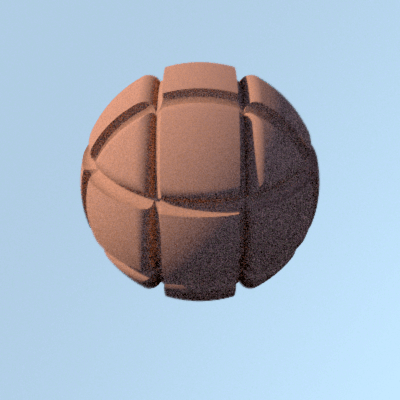
\includegraphics[width=.5\linewidth]{img/2 art/example_scene.png}
	\caption{Example scene in ART: a grooved sphere illuminated by the Wilkie-Hosek sky model \cite{hosek2012analytic}.}
	\label{fig:art_scene}
\end{figure}



